\subsection{Soldering}
\begin{figure}[h]
  \centering
  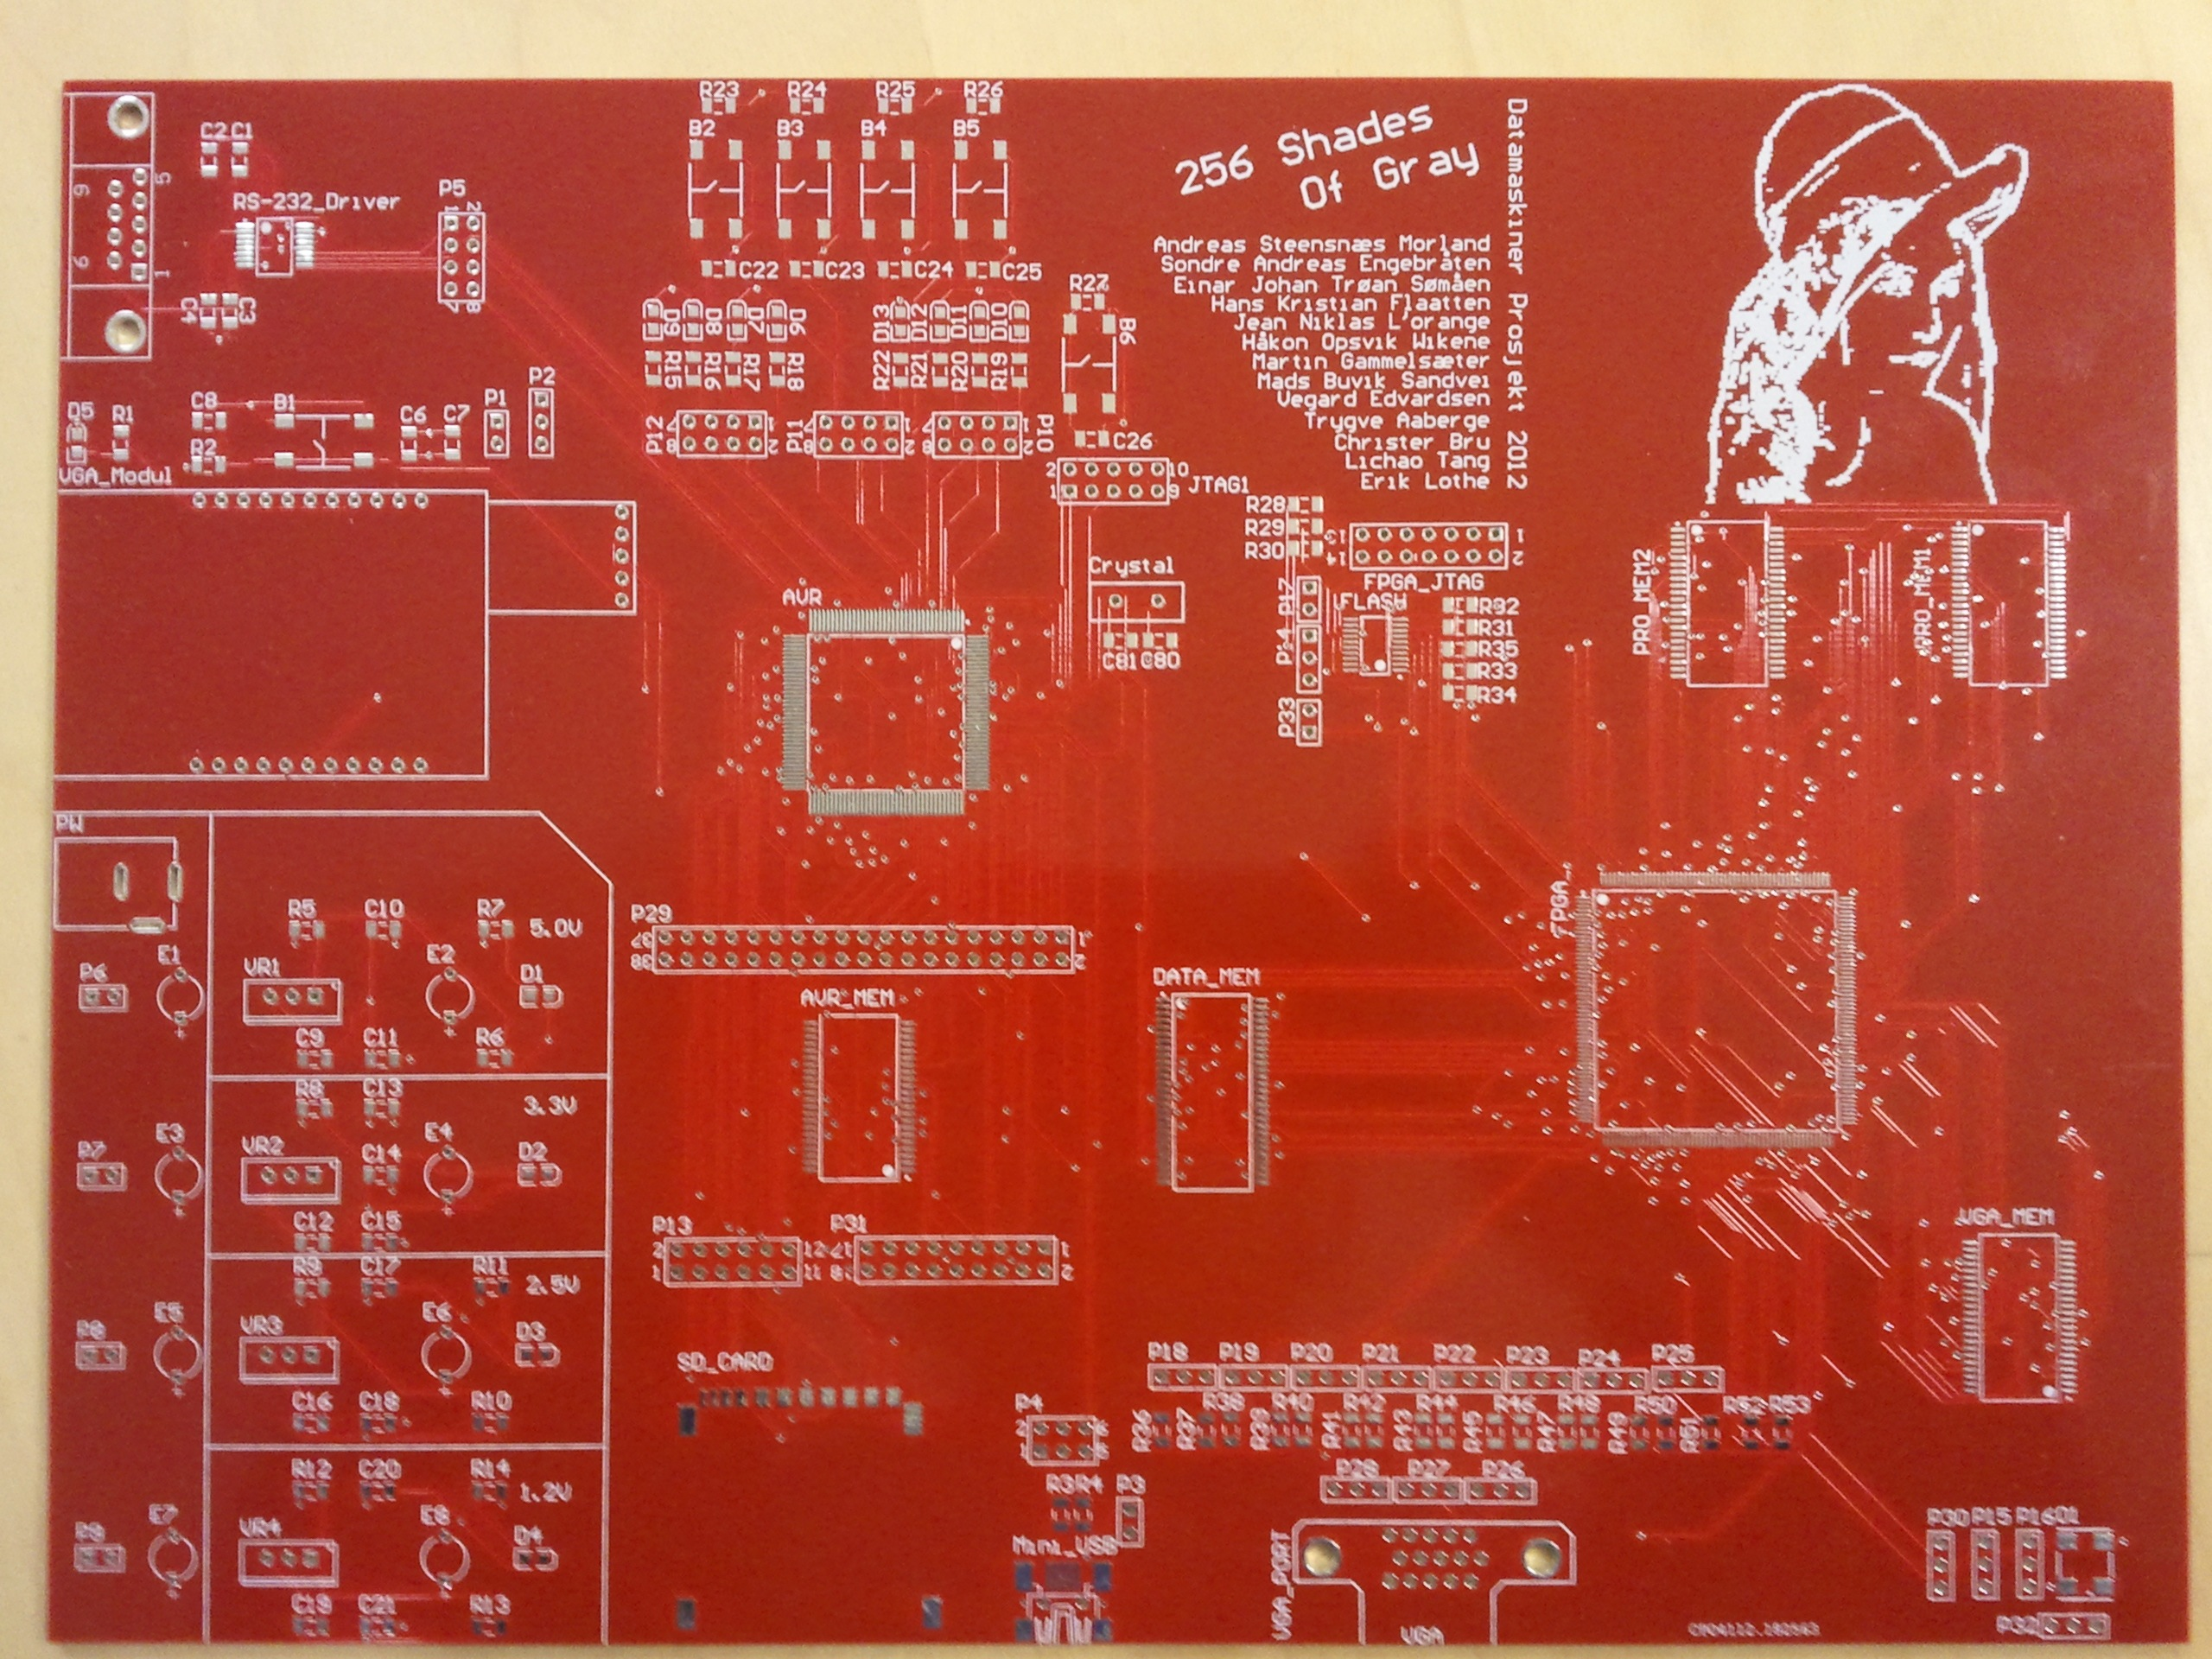
\includegraphics[width=0.8\textwidth]{fig/pcb/pcbwithoutcomp.jpg}
  \caption{The PCB Without Components}
  \label{fig:pcb-without-components}
\end{figure}


When the \ac{PCB} arrived from production, the soldering proved
to be a bit more difficult than originally anticipated.
First, we tested whether
there were any short circuits in the board itself. We used the multimeter to test that
there was no current passing from one layer to another. Then, we started to solder the power supply, one power plane at time, testing the board for short
circuit after each iteration. The table \ref{fig:pcb} shows the observed voltage from each plane.

\begin{table}[h]
  \centering
  \begin{tabularx}{\textwidth}{l l l l}\toprule
    \thx{Test} & \thx{Result} & \thx{Passed} 
    \\ 
	 \midrule
    Power supply 12.0V               &Measured 12.045  & OK  \\	
\midrule
    Power supply 5.0V               &Measured 4.995  & OK  \\
    \midrule
    Power supply 3.3V                   & Measured 3.286 & OK  \\
    \midrule
    Power supply 2.5V                 & Measured 2.510 & OK \\
    \midrule
    Power supply 1.2V            & Measured 1.240 & OK  \\
    
    \bottomrule
  \end{tabularx}
  \caption{Results of power supply}
  \label{fig:pcb}
\end{table}


\begin{figure}[h]
  \centering
  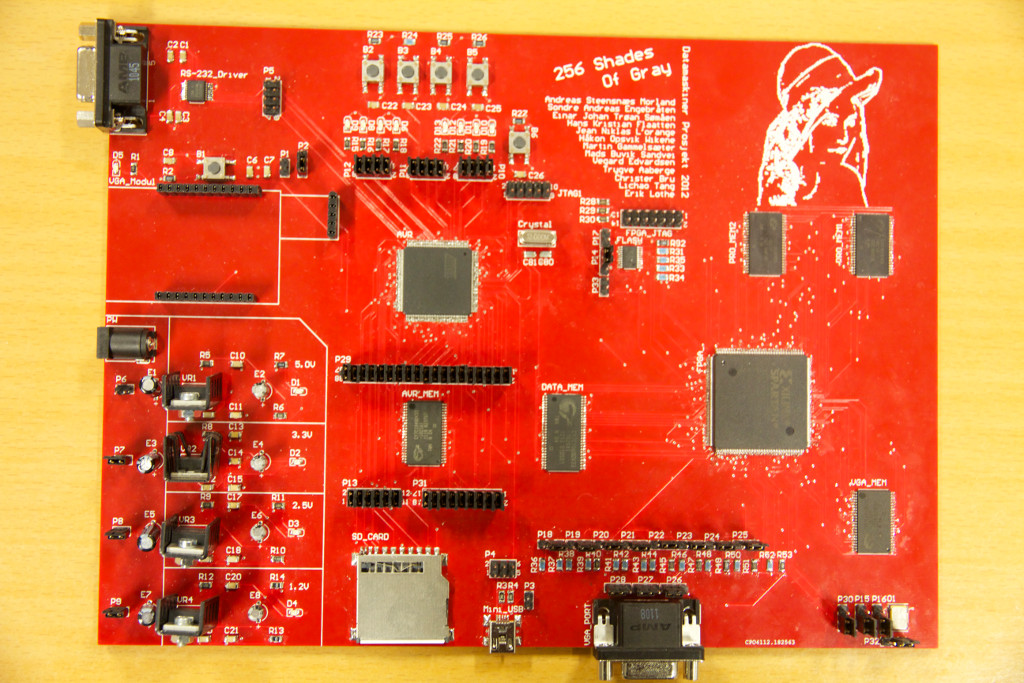
\includegraphics[width=0.8\textwidth]{fig/pcb/pcbwithcompnew.jpeg}
  \caption[The PCB]{The PCB With All The Components.}
  \label{fig:pcb-with-components}
\end{figure}


After about a days work we managed to completely destroy a pin on the AVR,
therefore we had to start soldering a new board. On this new board we
started soldering the AVR and \ac{FPGA}, as they were the hardest components to
solder on the first board. After soldering each side on the AVR and \ac{FPGA}, 
we tested the board for short circuits. As no short circuits were found, 
we moved on to soldering the power supply, as well as the \acp{JTAG}, FLASH 
and \acp{LED}. In order to check that the \ac{PCB} was working, the
AVR and \ac{FPGA} groups tested the \ac{PCB} without the capacitors. 
After both groups had tested that they could connect to the AVR and \ac{FPGA}
respectively, we soldered the rest of the \ac{PCB}.
